\documentclass[11pt]{article}
\usepackage[a4paper,  margin=1in]{geometry}
\usepackage{enumitem}
\usepackage{color}
\usepackage{graphicx}
\usepackage{caption}
\usepackage{subcaption}
\usepackage{algorithm}
\usepackage{algorithmicx}
\usepackage{algpseudocode}
\usepackage{listings}
\usepackage{amssymb}
\usepackage{tikz}
\usepackage{pgfplots}

\definecolor{dkgreen}{rgb}{0,0.6,0}
\definecolor{gray}{rgb}{0.5,0.5,0.5}
\definecolor{codebg}{rgb}{0.95,0.95,0.9}
\definecolor{mauve}{rgb}{0.58,0,0.82}

\lstset{frame=tb,
  rulecolor=\color{codebg},
  backgroundcolor=\color{codebg},
  language=C++,
  aboveskip=3mm,
  belowskip=-0.5mm,
  showstringspaces=false,
  columns=flexible,
  basicstyle={\small\ttfamily},
  numbers=none,
  numberstyle=\tiny\color{gray},
  morekeywords={vector},
  keywordstyle=\color{blue},
  commentstyle=\color{dkgreen},
  stringstyle=\color{mauve},
  breaklines=true,
  breakatwhitespace=true,
  tabsize=3
}

\graphicspath{{pic/}}
\setlength\parskip{6pt}
\setlength\parindent{0pt}
\setlength\intextsep{9pt}
\linespread{1}
\renewcommand{\refname}{\vspace{-30pt}}
\renewcommand\floatpagefraction{0.85}
\newcommand*{\equal}{=}

\title{\bf{VFX Project 1\\\large{High Dynamic Range Imaging}}\vspace{-10pt}}
\author{B03901056 Fan-Keng Sun, B03901119 Shang-Wei Chen}
\date{}
  
\begin{document}
\maketitle
\section{Description}
In this project, we assemble high dynamic range (HDR) images from a series of photographs under various exposures, using a popular vision library, OpenCV, for image processing and I/O. The photographs are preprocessed using median threshold bitmap (MTB) algorithm for image alignment. With the aid of tone mapping algorithm, HDR images are reproduced to LDR images in a better human perceptual sense. We learned basic photographing theories and image processing skills from the project. The features we have implemented are:
\vspace{-8pt}
\begin{itemize}
  \itemsep=-2pt
  \item Image alignment: MTB algorithm.
  \item HDR imaging: Paul Debevec's method.
  \item Tone mapping: Erik Reinhard's method.
  \item Exposure fusion: Tom Mertens' method.
  \item Blob removal
  \item Ghost removal: EA Khan's method.
  \item Spotlighting
\end{itemize}
\vspace{-8pt}

\section{Implementation}
\subsection{Environment}
\begin{itemize}
  \itemsep=-2pt
  \item Camera: Sony A6000 (lens: Sony SELP1650)
  \item OS: Linux (Archlinux 4.10, Ubuntu 16.04)
  \item Tools/Libraries: gcc/g++ 6.3.1, OpenCV 3.2 (C++), Boost $>=$ 1.5, Cmake $>=$ 3.0
\end{itemize}

\subsection{Image alignment}
Before HDR processing, image alignment is involved for better performance. The algorithm we used is shown in \textbf{Algorithm 1}, which is an implementation of \textbf{median threshold bitmap (MTB) algorithm} \cite{ref:Ward}. The function 

\begin{lstlisting}
  void MTB::process(vector<Mat>& res)
\end{lstlisting}

takes \texttt{cv::Mat} images for input and pass the result by reference. The alignment function transforms these images to 8-bit grayscale ones, while the others may approximately use only the green channel since this channel is higher weighted when converting color. Applying multi-scale techniques, we then form a pyramid of each grayscale photo in which the photos are scaled by a factor of two in each dimension. Consequently, filtering the photos to generate bitmaps thresholded by the median in each photo; thus, the bitmaps can be viewed as black-and-white photos. We can compute the amount of differences between two bitmaps using bitwise XOR, and find the optimal way to shift photos. Finally, scale these photos to crop the blank pixels on the edges resulted from shifting. There might be noisy areas at which the pixel luminance is close to the median; hence, adding a mask to exclude these areas may help following alignment processes. These features are realized by the following functions:

\begin{lstlisting}
  void MTB::transform_bi(const Mat& m, Mat& bi, Mat& de, int max_denoise)
  void MTB::shift(Mat& m, Mat& dst, const pair<int, int>& diff)
  pair<int, int> MTB::align(const int j, int lev, const int max_level)
\end{lstlisting}

One may refer to \texttt{src/mtb.hpp} and \texttt{src/mtb.cpp} for more details. 

\begin{algorithm}
\caption{MTB algorithm \cite{ref:Ward}}
\begin{algorithmic}[1]
\State $pics\gets$ images read via OpenCV
\State $max\_level\gets$ user parameter for aligning iterations
\State $max\_denoise\gets$ user parameter for setting noise area
\Function{MtbProcess}{$pics, max\_level, max\_denoise$}
	\State $N\gets$ number of $pics$
	\State $bi\_pics, masks\gets$ new image array with dimension $N$ and $max\_level$
	\For{$i$ in range($N$)}
		\State $p\gets pics[i]$
		\For{$j$ in range($max\_level$)}
			\State \Call{MtbTransformBi}{$p, bi\_pics[N][j], masks[N][j], max\_denoise$}
			\State $pic\gets pic$ with half size
		\EndFor
	\EndFor
	\State $offsets\gets$ array of size $N$
	\ForAll{$i$ in range($N$)}
		\State $offsets[i]\gets$\Call{MtbAlign}{i, 0, $max\_level$}
	\EndFor
	\State Shift $pics$ with $(xshift, yshift)$ pairs in $offsets$
	\State Scale $pics$ to crop blank pixels
\EndFunction
\Statex
\Function{MtbTransformBi}{$p, bi, de, max\_denoise$}
	\State $bi, de\gets p$ converted to gray scale
	\State $m\gets$ median value of all pixel in $bi$
	\ForAll{pixel $i$ in $bi$}
		\If{$i.value<m$}
			\State $i.value\gets gray.value.min$
		\Else
			\State $i.value\gets gray.value.max$
		\EndIf
	\EndFor
	\ForAll{pixel $i$ in $de$}
		\If{$i.value<m-max\_denoise$ or $i.value>m+max\_denoise$}
			\State $i.value\gets gray.value.max$
		\Else
			\State $i.value\gets gray.value.min$
		\EndIf
	\EndFor
\EndFunction
\algstore{algmtb}
\end{algorithmic}
\end{algorithm}

\begin{algorithm}
\begin{algorithmic}[1]
\algrestore{algmtb}
\Function{MtbAlign}{$i, level, max\_level$}
	\If{$level$ equals $max\_level$}
		\State \Return{$(0, 0)$}
	\EndIf
	\State $(xshift, yshift)\gets$\Call{MtbAlign}{$i, level+1, max\_level$}
	\Comment{Call this function recursively}
	\State $fixed, moved\gets bi[0][level], bi[i][level]$
	\Comment{Align $pic[i]$ to $pic[0]$}
	\State $mask\_f, mask\_m\gets masks[0][level], masks[i][level]$
	\For{$xshift, yshift$ in $[-1, 0, 1]$}
		\State $moved\_sh\gets moved$ with $(xshift, yshift)$
		\State $cnt_k\gets$ \# of diff between $fixed$ and $moved\_sh$
without $mask\_f$ and $mask\_m$ area	
	\EndFor
	\State $(xshift\_best, yshift\_best)\gets(xshift, yshift)$ with min\{$cnt_k$\}
	\State\Return$(xshift*2+xshift\_best, yshift*2+yshift\_best)$
\EndFunction
\end{algorithmic}
\end{algorithm}
\subsection{HDR Imaging}
In our project, we have implemented two methods for HDR imaging: \textbf{Paul Debevec's method} \cite{ref:debevec} and \textbf{Tom Mertens' method} \cite{ref:mertens} (referred to \textbf{Algorithm 2} and \textbf{Algorithm 3}, respectively).

As mentioned in the class, we construct matrix $A$ and vector $\textbf{b}$, and then compute the solution of $\textbf{x}$ to $A\textbf{x}=\textbf{b}$, where the indice of $A$ and $\textbf{b}$ are calculated from the aligned photos combined with a hat weighting function. Once the response curve recovery is done, we can construct the high dynamic range radiance map according to \cite{ref:debevec}
$$\ln E_i=g(Z_{ij})-\ln\Delta t_j$$
For robustness, we choose to reduce noise in the result using the following function rather than the above one
$$\ln E_i=\frac{\sum_{j=1}^P w(Z_{ij})(g(Z_{ij}-\ln\Delta t_j))}{\sum_{j=1}^Pw(Z_{ij})}$$
Debevec's method is realized in 
\begin{lstlisting}
  void DEBEVEC::process(
    const vector<Mat>& pics, 
    const vector<double>& etimes, 
    const vector<Mat>& gW, 
    Mat& result
  )
\end{lstlisting}
in which the parameter \texttt{gW} is involved for \textbf{ghost removal} feature. We will discuss it in the following sections.

\begin{algorithm}
\caption{HDR algorithm using Paul Debevec's method \cite{ref:debevec}}
\begin{algorithmic}[1]
\State $etimes\gets$ exposure time of each photos
\State $lambda\gets$ user parameter for smoothness
\State $nSample\gets$ user parameter for amount of sampling points
\State $nPics\gets$ number of photos in $pics$
\State $points\gets nSample$ points randomly from $pics[0]$

\Function{HdrDebevec}{$pics, etimes$}
  \State $w\gets$ hat weighting function with min $=1$ and max $=128$
\algstore{deb}
\end{algorithmic}
\end{algorithm}

\begin{algorithm}
\begin{algorithmic}[1]
\algrestore{deb}
  \For{$ch$ in range(3)}
    \State $X[ch]\gets$ new array of size 256
    \State $A\gets$ new array of zeros with size $(nSample*nPics+257)\times(nSample+256)$
    \State $B\gets$new array of zeros with size $(nSample*nPics+257)\times 1$
    \State $k\gets 0$
    \For{$i$ in range($nSample$)}
      \For{$j$ in range($nPics$)}
        \State $val\gets pics[point[i]]$
        \State $A[k][val]\gets w[val]$
        \State $A[k][256+i]\gets-w[val]$
        \State $B[k][0]\gets w[val]*\log(etimes[j])$
        \State $k\gets k+1$
      \EndFor
    \EndFor
    \State $A[k][128]\gets 1$
    \For{$i$ in range(254)}
      \State $k\gets k+1$
      \State $A[k][i]\gets lambda*w[i]$
      \State $A[k][i+1]\gets -2*lambda*w[i]$
      \State $A[k][i+2]\gets lambda*w[i]$
    \EndFor
    \State $X[ch]\gets (A/B)$[0 to 255]
  \EndFor	
  \For{$ch$ in range(3)}
    \For{pixel $i$ in a photo of channel $ch$)}
      \State $nom\gets$ sum\{$w[i.value]*(pics[p][i.value]-\log(etimes[j]))$ for each photo $pics[p]$\}
      \State $denom\gets$ sum\{$w[i.value]$ for each photo $pics[p]$\}
      \State $res[ch][i]\gets\exp(nom/denom)$
    \EndFor
  \EndFor
  \State\Return $res$
\EndFunction
\end{algorithmic}
\end{algorithm}

\newpage 
For Mertens' method \cite{ref:mertens}, \textbf{exposure fusion}, the algorithm keeps the best parts of each photos under various exposure realizing with weighted blending. In the first part, we compute some quality measures, \textbf{contrast}, \textbf{saturation}, and \textbf{well-exposedness}, for the purpose of producing a weighting function.
$$ W_{ij,k}=(C_{ij,k})^{\omega_C}*(S_{ij,k})^{\omega_S}*(E_{ij,k})^{\omega_E} $$
in which the qualities, contrast ($C$), saturation ($S$), and well-exposedness ($E$) are given with different weighting exponents $\omega_C$, $\omega_S$, and $\omega_E$, respectively. 
In the next part, fusion, we compute $N$ normalized weight maps from above quantities
$$\hat{W}_{ij,k}= \left[ \sum_{k'=1}^N W_{ij,k'} \right]^{-1}{W}_{ij,k}$$
The method then compute Laplacian pyramids and Gaussian pyrymids of the input images. Summing up their product of each photos to obtain the fused pyramid, we can recover the final image:
$$ \textbf{L}\{R\}^l_{ij}=\sum_{k=1}^N\textbf{G}\{\hat{W}\}^l_{ij,k}\textbf{L}\{I\}^l_{ij,k} $$
where $R$ stands for the result image, and $l$ for the level of pyramids. Finally, collapse the Laplacian pyramids to obtain HDR result. Mertens' method is realized in 
\begin{lstlisting}
  void MERTENS::process(
    const vector<Mat>& pics,
    const vector<Mat>& gW, 
    Mat& result
  )
\end{lstlisting}
One may refer to \texttt{src/hdr.hpp} and \texttt{src/hdr.cpp} for more details.

\begin{algorithm}
\caption{HDR algorithm using Tom Mertens's method \cite{ref:mertens}}
\begin{algorithmic}[1]
\State $wC, wS, wE\gets$ user parameters for weighting functions
\State $max\_level\gets$ user parameter for building pyramids
\Function{HdrMertens}{$pics$}
  \State $nPics\gets$ number of photos in $pics$
  \State $sPics\gets pics$ where the value of pixels are scaled from int 0-255 to float number 0-1
  \For{$i$ in range($nPics$)}
    \State $grayPic\gets$ convert $sPics[i]$ to gray scale 
    \State $C\gets$ abs(\Call{LapacianFilter}{$grayPic$})
    \State $S\gets$ standard\_deviation(values of pixels in three channels of $sPics[i]$)
    \State $E\gets$ \Call{GaussCurve}{$sPics[i].pixel.intensity-0.5$, $\sigma=0.2$}
    \State $W\gets \mbox{pow}(C, wC) *\mbox{pow}(S, wS) *\mbox{pow}(E, wE)$
  \EndFor
  \State $W\gets W/$sum\{$W$\}
  \State $pyrPics\gets$ \Call{BuildPyramid}{$sPics$}
  \State $pyrW\gets$ \Call{BuildPyramid}{$W$}
  \State $pyrRes\gets$ pyramid of zeros with the same shape of $pyrPics$
  \State $picUp\gets$ new image
  \For{$i$ in range($nPics$)}
    \For{$j$ in range($max\_level$)}
      \State \Call{PyramidUp}{$pyrPics[i][j+1]$, $picUp$, $pyrPics[i][j].size$}
      \State $pyrPics[i][j]\gets pyrPics[i][j]-picUp$
    \EndFor
    \For{$j$ in range($max\_level+1$)}
      \State $pyrPics[i][j]\gets pyrPics[i][j]*pyrW[i][j]$
      \State $pyrRes[j]\gets pyrRes[j]+pyrPic[i][j]$ 
    \EndFor
  \EndFor
  \For{$i$ from $max\_level$ to 0}
    \State \Call{PyramidUp}{$pyrRes[i+1]$, $picUp$, $pyrPics[i][j].size$}
    \State $pyrRes[i]\gets pyrRes[i]+picUp$
  \EndFor
  \State \Return $pyrRes[0]$
\EndFunction
\end{algorithmic}
\end{algorithm}


\subsection{Tone Mapping}
We realize this part by \textbf{Erik Reinhard's method} \cite{ref:tone-map}, which is shown in \textbf{Algorithm 4}. The algorithm we used is an inspiration from photoreceptor physiology, which can be separated into two concepts: global and local reproduction. The part of global operators considers overall characteristics, such as contrast, brightness, color saturation, and etc., for visual perceptions. On the other hand, the part of local operators focuses on local modifications, such as haloing and ringing.
\begin{lstlisting}
  void TONEMAP::process(Mat& input, Mat& output)
\end{lstlisting}
One may refer to \texttt{src/tonemap.hpp} and \texttt{src/tonemap.cpp} for more details.

\begin{algorithm}
\caption{Tone mapping algorithm \cite{ref:tone-map}}\label{euclid}
\begin{algorithmic}[1]
\State $f\gets$ user parameter for intensity
\State $m\gets$ user parameter for contrast
\State $a\gets$ user parameter for light adaption 
\State $c\gets$ user parameter for chromatic adaption
\Function{Tonemap}{$image\_in$, $image\_out$}
\State $L\_map\gets$ luminance of each pixel in $image\_in$
\State $Cav[3]\gets$ mean value of each channels of $image\_in$
\State $Lav\gets$ mean value of $L\_map$
\State $L\_min\gets$ minimal value in $L\_map$
\State $L\_max\gets$ maximal value in $L\_map$
\ForAll{channel $n$ of $image\_in$}
\ForAll{pixel $i$ in $image\_in[n]$}
\State $L\gets$ value of the same position in $L\_map$
\State $I\_local\gets c* image\_in[n][i]+ (1-c)*L$
\State $I\_global\gets c*Cav[n]+ (1-c)* Lav$
\State $I\_adaption\gets a*I\_local+(1-a)*I\_global$
\State $image\_out[n][i]\gets image\_in[n][i]/(image\_in[n][i]+\mbox{pow}(f*I\_adaption, m))$
\EndFor
\EndFor
\State Normalize the value of pixels in $image\_out$ to an integer in the range from 0 to 255
\EndFunction
\end{algorithmic}
\end{algorithm}



\subsection{Blob Removal}
Owing to imperfection of original photos or some irregular situations that the above algorithms do not handle, there might be blobs on the photos. We implement blob removal based on a feature in OpenCV libraries, \texttt{cv::SimpleBlobDetector}. Using the following function (need to include \texttt{features2d.hpp})
\begin{lstlisting}
  static Ptr<SimpleBlobDetector> cv::create(
    const SimpleBlobDetector::Params &parameters=SimpleBlobDetector::Params()
  )
\end{lstlisting}
simply convert RGB color to gray scale only, which may not detect the blobs completely; what's more, splitting RGB color into three channels and thresholding by each channel are not effective enough. Hence, we transform RGB color to \textbf{Lab color space} and threshold the image by \textbf{L} (lightness), \textbf{a} (green-red color component), and \textbf{b} (blue-yellow color component) channels separately, which may have better performance for blob detection, and then use the original \texttt{cv::SimpleBlobDetector} functions to detect the blobs.

This feature is realized by the following function in \texttt{src/util.cpp}
\begin{lstlisting}
  void blob_removal(const Mat& pic, Mat& result)
\end{lstlisting}
Since \texttt{cv::SimpleBlobDetector} provides many parameters for blob detection, such as blob size, circularity, inertia ratio, convexity, and for convenience, we create a panel for tuning these parameters (Fig. \ref{fig:blob-panel}). One of the advantages is that we can manually figure out the correctness of blob detection, and thus prevent the detection from some unwanted results if performing automatically. However, iterations is required for completeness since different blobs may have their own threshold values.

\begin{figure}[!ht]
  \centering
  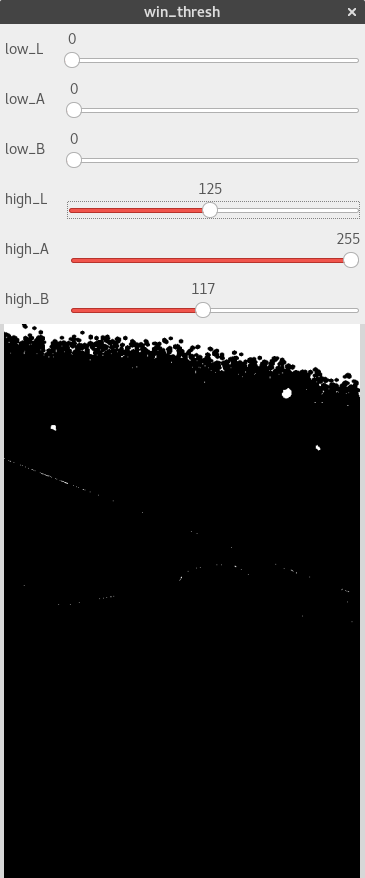
\includegraphics[height=16cm]{blob-panel1}
  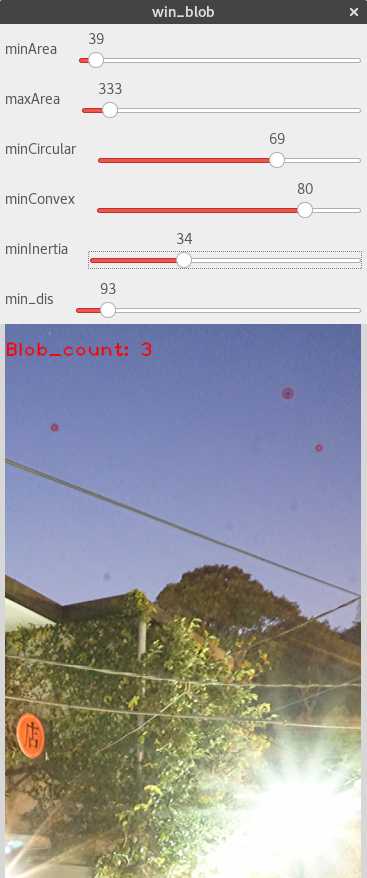
\includegraphics[height=16cm]{blob-panel2}
  \caption{Panel for blob removal}
  \label{fig:blob-panel}
\end{figure}

Once the blobs are detected, we approximately fill out these areas with the average colors nearby. For more details, one can refer to \texttt{src/util.hpp} and \texttt{src/util.cpp}. 
\subsection{Ghost Removal}
The feature is realized in the following function
\begin{lstlisting}
  void ghost_removal(const vector<Mat>& pics, int iter, vector<Mat>& result)
\end{lstlisting}
which is an implementation of \textbf{EA Khan's method} \cite{ref:ghost-removal}. The algorithm iteratively calculate the possibility of each pixel based on its weight, and then calculate the weight for the next iteration by its possibility. For a series of $R$ photos under different exposure times, we assign a vector $\textbf{x}_{ijr}=(L, a, b, i, j)\in \mathbb{R}^5$ to each pixel on a photo, where $L$, $a$, $b$ represent its color, $i$, $j$ represent its position, and $r$ represents the number of photo that contains it. Define the neighborhood of the vector $\textbf{x}_{ijr}$
$$F=\{ \textbf{y}_{pqs}|(p,q,s)\in\textbf{N}(\textbf{x}_{ijr}), (p,q)\neq(i,j), s=1,2,\cdots,R \}$$
In the first iteration, define the weight by a hat function (Fig. \ref{fig:hat})
$$w(Z)=1-\left(2\cdot\frac{Z}{255}-1\right)^{12}$$

\begin{figure}[!ht]
\center
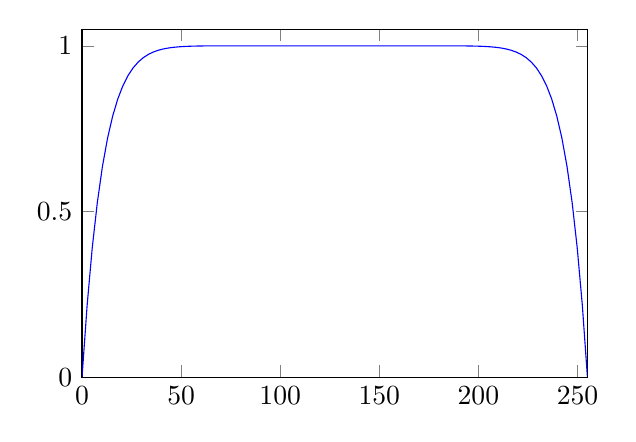
\begin{tikzpicture}
  \begin{axis}[
    domain=0:255,
    xmin=0, xmax=255,
    ymin=0, ymax=1.05,
    samples=100,
    width=8cm, height=6cm
  ]
    \addplot+[mark=none] {1-(2*(x/255)-1)^12};
  \end{axis}
\end{tikzpicture}
\caption{Hat function for ghost removal weighting}
\label{fig:hat}
\end{figure}

where $Z$ is the average value of three channels. Then, calculate the possibility by
$$ 
P(\textbf{x}_{ijr}|F)=
\frac{
  \sum_{p,q,s\in N(\textbf{x}_{ijr})}w_{pqs}K_\textbf{H}(\textbf{x}_{ijr}-\textbf{y}_{pqs})
  }{
    \sum_{p,q,s\in N(\textbf{x}_{ijr})}w_{pqs}
  } 
$$
where
$$K_\textbf{H}(\textbf{x})=|\textbf{H}|^{-1/2}(2\pi)^{-5/2}\exp(-\frac{1}{2}\textbf{x}^T\textbf{H}^{-1}\textbf{x})$$
and $\textbf{H}$ is an identity matrix. Afterwards, calculate the weight for the next iteration
$$w_{pqs, t+1}=w(Z_s(p,q))\cdot P(\textbf{x}_{ijr}|F)$$
in which $w(Z_s(p,q))$ stands for the initial weight.


\subsection{Spotlighting}
Since there might be some objects moving irregularly when shooting photographs, and can barely rebuild the image by the previous ghost removal method, we use the function
\begin{lstlisting}
  void cv::seamlessClone(InputArray src, InputArray dst, InputArray mask, Point p, OutputArray blend, int flags)
\end{lstlisting}
in OpenCV libraries to recover the waving parts in the photos by simply replacing them based on one photo. The feature is realized in the following function
\begin{lstlisting}
  void add_spotlight(vector<Mat>& pics, const vector<double>& para)
\end{lstlisting}
One may refer to \texttt{src/util.cpp} for more detail.

\section{Results}
\subsection{Response Curve}
The recovered response curves are shown in Fig. \ref{fig:response-curve}, where the smoothness parameter $\lambda$ is varied.
\begin{figure}[!ht]
\center
\hspace{-45pt}
\begin{tikzpicture}
  \begin{axis}[
    domain=0:255,
    xlabel=pixel value ($\lambda\equal 0.5$),
    xlabel style={font=\scriptsize},
    ylabel=log exposure,
    ylabel near ticks,
    ylabel style={font=\scriptsize},
    xticklabel style={font=\scriptsize},
    yticklabel style={font=\scriptsize},
    xmin=0, xmax=255,
    ymin=-4.5, ymax=3,
    samples=100,
    width=6cm, height=5cm
  ]
  \addplot [color=blue, thick] table [x=x, y=y] {data/curveB_0.5.txt};
  \addplot [color=red, thick] table [x=x, y=y] {data/curveR_0.5.txt};
  \addplot [color=green, thick] table [x=x, y=y] {data/curveG_0.5.txt};
  \end{axis}
\end{tikzpicture}
\begin{tikzpicture}
  \begin{axis}[
    domain=0:255,
    xlabel=pixel value ($\lambda\equal 5$),
    xlabel style={font=\scriptsize},
    xticklabel style={font=\scriptsize},
    yticklabel style={font=\scriptsize},
    xmin=0, xmax=255,
    ymin=-4.5, ymax=3,
    samples=100,
    width=6cm, height=5cm
  ]
  \addplot [color=blue, thick] table [x=x, y=y] {data/curveB_5.txt};
  \addplot [color=red, thick] table [x=x, y=y] {data/curveR_5.txt};
  \addplot [color=green, thick] table [x=x, y=y] {data/curveG_5.txt};
  \end{axis}
\end{tikzpicture}
\begin{tikzpicture}
  \begin{axis}[
    domain=0:255,
    xlabel=pixel value ($\lambda\equal 50$),
    xlabel style={font=\scriptsize},
    xticklabel style={font=\scriptsize},
    yticklabel style={font=\scriptsize},
    xmin=0, xmax=255,
    ymin=-4.5, ymax=3,
    samples=100,
    width=6cm, height=5cm
  ]
  \addplot [color=blue, thick] table [x=x, y=y] {data/curveB_50.txt};
  \addplot [color=red, thick] table [x=x, y=y] {data/curveR_50.txt};
  \addplot [color=green, thick] table [x=x, y=y] {data/curveG_50.txt};
  \end{axis}
\end{tikzpicture}
\hspace{-45pt}
\caption{Response curve for Sony A6000}
\label{fig:response-curve}
\end{figure}



\begin{figure}[!ht]
  \centering
  %\subcaptionbox{Ponzo illusion\vspace{5pt}}{\includegraphics[width=.3\linewidth]{blob-panel}}
  %\caption{782\cite{ref:optical-illusion}}
  \label{distort}
\end{figure}

\section{Reference}
\bibliographystyle{unsrt}
\bibliography{hw1}
\end{document}
